\documentclass{article}
\usepackage{tikz}
\usepackage{amsmath}

\begin{document}

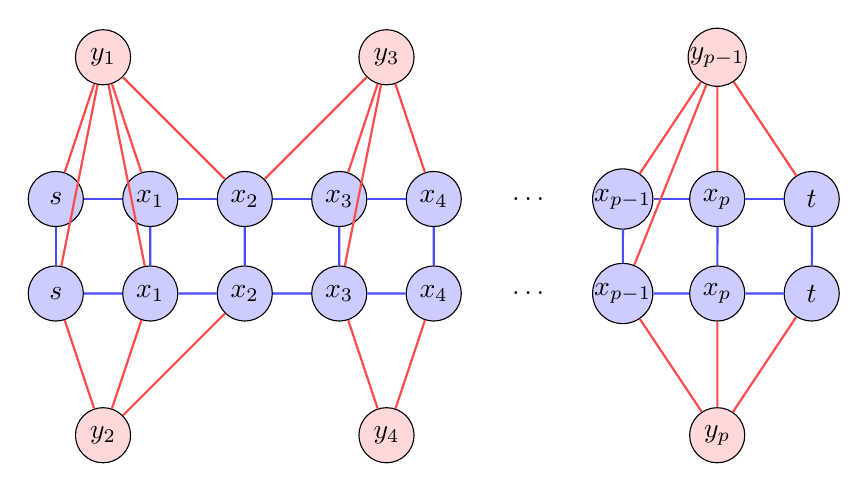
\begin{tikzpicture}[
    scale=1.2,
    vertex/.style={circle, draw, minimum size=0.7cm, inner sep=0pt},
    blue vertex/.style={vertex, fill=blue!20},
    red vertex/.style={vertex, fill=red!15},
    blue edge/.style={draw, blue!70, thick},
    red edge/.style={draw, red!70, thick}
]

% Blue vertices (original graph H)
% First row
\node[blue vertex] (s) at (0,0) {$s$};
\node[blue vertex] (x1) at (1,0) {$x_1$};
\node[blue vertex] (x2) at (2,0) {$x_2$};
\node[blue vertex] (x3) at (3,0) {$x_3$};
\node[blue vertex] (x4) at (4,0) {$x_4$};
\node at (5,0) {$\ldots$};
\node[blue vertex] (xp1) at (6,0) {$x_{p-1}$};
\node[blue vertex] (xp) at (7,0) {$x_{p}$};
\node[blue vertex] (t) at (8,0) {$t$};

% Second row
\node[blue vertex] (s2) at (0,-1) {$s$};
\node[blue vertex] (x12) at (1,-1) {$x_1$};
\node[blue vertex] (x22) at (2,-1) {$x_2$};
\node[blue vertex] (x32) at (3,-1) {$x_3$};
\node[blue vertex] (x42) at (4,-1) {$x_4$};
\node at (5,-1) {$\ldots$};
\node[blue vertex] (xp12) at (6,-1) {$x_{p-1}$};
\node[blue vertex] (xp2) at (7,-1) {$x_{p}$};
\node[blue vertex] (t2) at (8,-1) {$t$};

% Red vertices (additional vertices)
\node[red vertex] (y1) at (0.5,1.5) {$y_1$};
\node[red vertex] (y2) at (0.5,-2.5) {$y_2$};
\node[red vertex] (y3) at (3.5,1.5) {$y_3$};
\node[red vertex] (y4) at (3.5,-2.5) {$y_4$};
\node[red vertex] (yp1) at (7,1.5) {$y_{p-1}$};
\node[red vertex] (yp) at (7,-2.5) {$y_{p}$};

% Blue edges (original graph H)
\draw[blue edge] (s) -- (x1);
\draw[blue edge] (x1) -- (x2);
\draw[blue edge] (x2) -- (x3);
\draw[blue edge] (x3) -- (x4);
\draw[blue edge] (xp1) -- (xp);
\draw[blue edge] (xp) -- (t);

\draw[blue edge] (s2) -- (x12);
\draw[blue edge] (x12) -- (x22);
\draw[blue edge] (x22) -- (x32);
\draw[blue edge] (x32) -- (x42);
\draw[blue edge] (xp12) -- (xp2);
\draw[blue edge] (xp2) -- (t2);

\draw[blue edge] (s) -- (s2);
\draw[blue edge] (x1) -- (x12);
\draw[blue edge] (x2) -- (x22);
\draw[blue edge] (x3) -- (x32);
\draw[blue edge] (x4) -- (x42);
\draw[blue edge] (xp1) -- (xp12);
\draw[blue edge] (xp) -- (xp2);
\draw[blue edge] (t) -- (t2);

% Red edges (additional edges with weight |U|)
\draw[red edge] (y1) -- (s);
\draw[red edge] (y1) -- (x1);
\draw[red edge] (y1) -- (x2);
\draw[red edge] (y1) -- (s2);
\draw[red edge] (y1) -- (x12);

\draw[red edge] (y2) -- (s2);
\draw[red edge] (y2) -- (x12);
\draw[red edge] (y2) -- (x22);

\draw[red edge] (y3) -- (x2);
\draw[red edge] (y3) -- (x3);
\draw[red edge] (y3) -- (x4);
\draw[red edge] (y3) -- (x32);

\draw[red edge] (y4) -- (x32);
\draw[red edge] (y4) -- (x42);

\draw[red edge] (yp1) -- (xp1);
\draw[red edge] (yp1) -- (xp);
\draw[red edge] (yp1) -- (t);
\draw[red edge] (yp1) -- (xp12);

\draw[red edge] (yp) -- (xp12);
\draw[red edge] (yp) -- (xp2);
\draw[red edge] (yp) -- (t2);

\end{tikzpicture}

\end{document}